\documentclass[a4paper,12pt]{article}
\usepackage{cmap}
\usepackage[utf8]{inputenc}
\usepackage[warn]{mathtext}
\usepackage{epsf,amsmath,amsfonts,amssymb,amsbsy}
\usepackage[mathscr]{eucal}
\usepackage[english, russian]{babel}
\author{Толочко Константин Б03-205 }
\title{Лабораторная работа 3.2.5 (4.б)

Свободные и вынужденые колебания 

в электрическом контуре}
\usepackage[left=2cm,right=2cm,top=2cm,bottom=2cm]{geometry}
\usepackage{graphicx}
\usepackage{indentfirst}
\graphicspath{{pictures2.1.1/}}
\DeclareGraphicsExtensions{.pdf,.png,.jpg}
\usepackage{pgfplots}
\begin{document}
	\maketitle
	\begin{center}
	\end{center}
	\paragraph*{Цель работы:}исследование свободных и вынужденных колебаний в колебательном контуре.
	\paragraph*{В работе используются:}осциллограф AKTAKOM ADS-6142H, генератор сигналов специальной формы АКИП-3409/4, магазин сопротивления MCP-60, магазин емкости P5025, магазин индуктивности P567 типа МИСП, соединительная коробка с шунтирующей емкостью, соединительные одножильные и коаксиальные провода.
	\section{Теоретическое введение}

Условие реализации режима затухающих колебаний в $LCR$-контуре имеет вид\[0 < R < 2\sqrt{\frac{L}{C}}=R_{\text{кр}},\]где $R_{\text{кр}}$ -- \textit{критическое сопротивление}.

При выполнении этого условия напряжение $U_C(t)$ на конденсаторе зависит от времени как\[U_C(t)=U_0e^{-\gamma t}\cos{\left(\omega_1t+\varphi_0\right)}.\]Здесь $\gamma=\frac{R}{2L}$ - коэф. заухания, а $\omega_1=\sqrt{\frac{1}{LC}-\frac{R^2}{4L^4}}$  - круговая частота св. колебаний, где $\omega_1=\sqrt{{\omega_0}^2 - {\gamma}^2}$, а $\omega_0$ - собственная круговая частота кол-ий. 

Несложно заметить, что выражения для напряжения $U_C(t)$ и тока $I(t)$ можно при должном подборе начальной фазы записать в виде
\begin{flalign*}
&U_C(t)=U_{C0}e^{-\gamma t}\left(\cos{\omega_1t}+\frac{\gamma}{\omega_1}\sin{\omega_1t}\right),&&\\
&I(t)=C\dot{U}_C=-\frac{2U_{C0}}{R_{\text{кр}}}\frac{\omega_0}{\omega_1}e^{-\gamma t}\sin{\omega_1t}.&&
\end{flalign*}

С помощью этих формул можно параметрически представить \textit{траектории системы на фазовой плоскости} переменных $(U_C,I)$.

\begin{figure}[h]
	\centering
	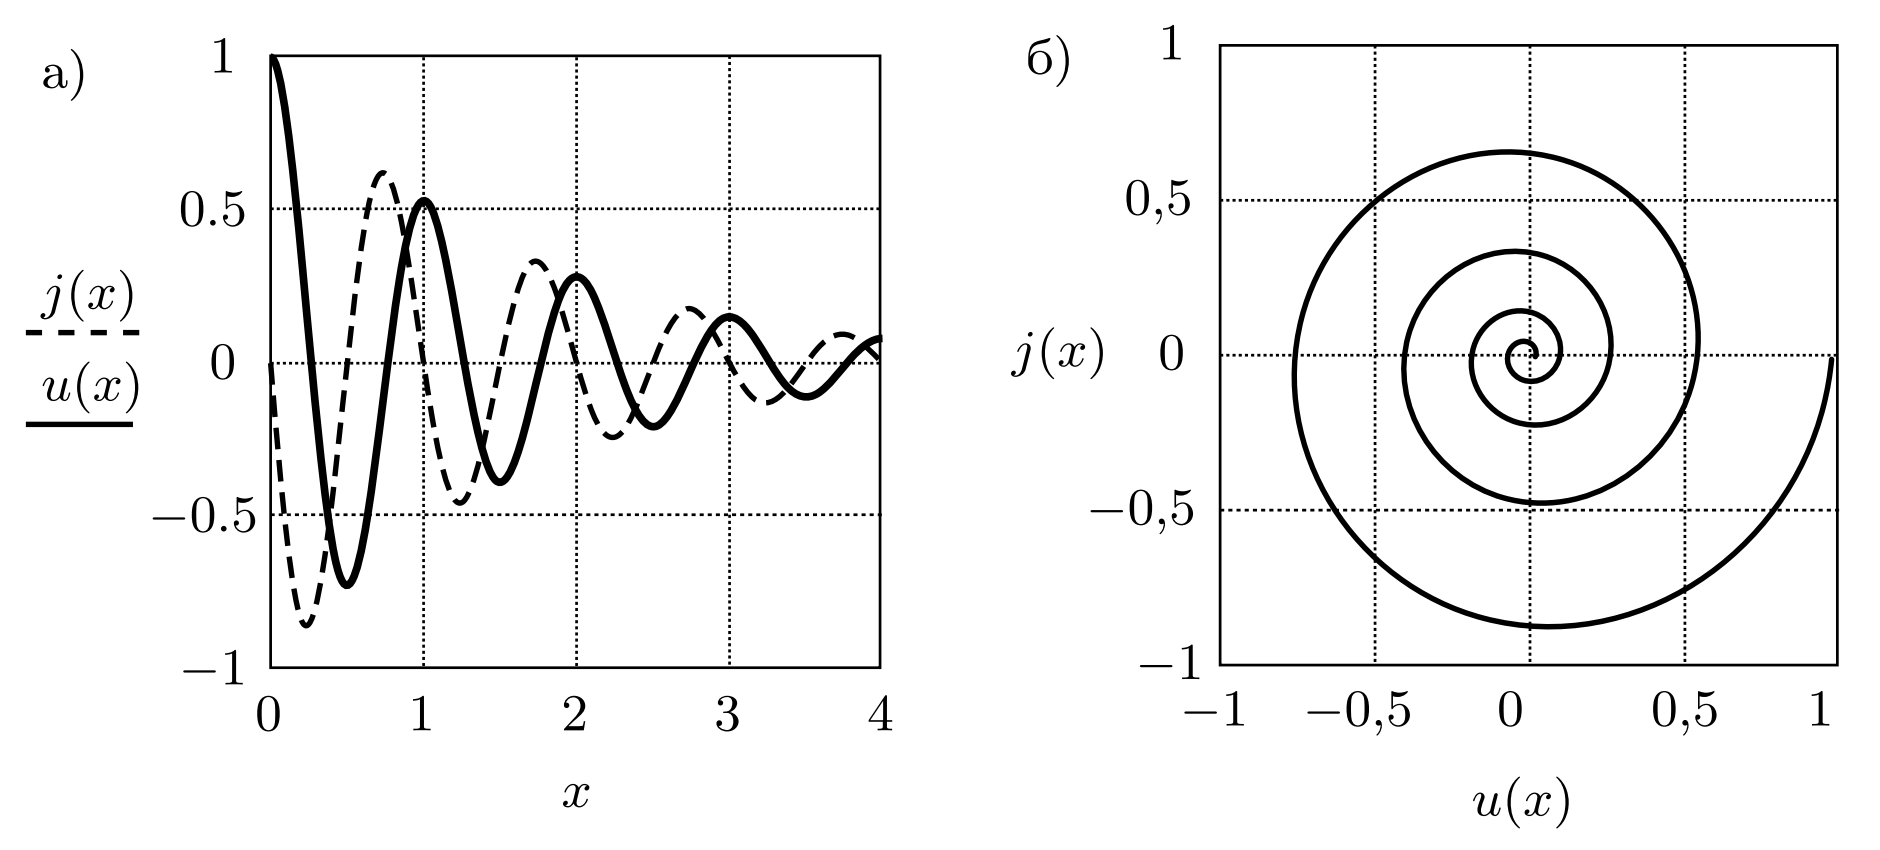
\includegraphics[scale=0.24]{th}
	\caption{Затухающие колебания: а) ток в контуре $j(x)$ и напряжение на конденсаторе $u(x)$, б) траектория системы на фазовой плоскости $(u,j)$} \label{th}
\end{figure}

\textit{Период затухающих колебаний} равен\[T_1=\frac{2\pi}{\omega_1} > T_0,\]т.е. наличие потерь в контуре приводит к увеличению периода колебаний.

Другими характеристиками процесса затухания являются \textit{время затухания}\[\tau=\frac{2L}{R},\] за которое амплитуда колебаний убывает в $e$ раз, и \textit{логарифмический декремент затухания}\[\Theta=\ln{\frac{U_k}{U_{k+1}}}=\gamma T_1,\]где $U_k$ и $U_{k+1}$ -- два последовательных максимума рассматрваемой величины.

С логарифмическим декрементом связана ещё одна важнейшая характеристика колебательного контура -- его \textit{добротность} $Q$:\[Q\equiv\frac{\pi}{\Theta}=\frac{1}{2}\sqrt{\frac{R_{\text{кр}}^2}{R^2}-1}.\]

При $Q\gg1$ можно с хорошей точностью заменить $\omega_1$ на $\omega_0$ в уравнениях для зависимости напряжения и тока в контуре от времени, что позволяет рассчитать теоретически добротность через параметры контура по формуле:
\begin{equation}\label{teor}
	Q = \frac{1}{R } \sqrt{\frac{L}{C}}
\end{equation}
\\
$$                                                             
$$
Вынужденые колебания в RLC-контуре представляют собой суперпозицию двух синусоид:
\begin{equation}
	I= B e^{-\gamma t} \sin (\omega t - \Theta)+ \frac{\mathcal{E}_0 \Omega}{L \rho_0} \sin (\Omega t - \psi),
	\label{law}
\end{equation}
При подключении контура к синусоидальной ЭДС собственные колебания с частотой $\omega$ со временем затухают. Однако при совпадении внешней частоты $ \Omega $ и собственной $ \omega $ возникает резонанс, при котором амплитуда вынужденных колебаний достигает максимального значения. Зависимость амплитуды установившихся колебаний от внешней частоты называется резонансной кривой.

Для достоверного исследования резонансной кривой необходимо, чтобы импеданс исследуемого участка цепи не зависел от импеданса источника питания даже на резонансе. С этой целью в работе используется параллельный колебательный контур (рис. \ref{fig:scheme})
\begin{figure}
	\centering
	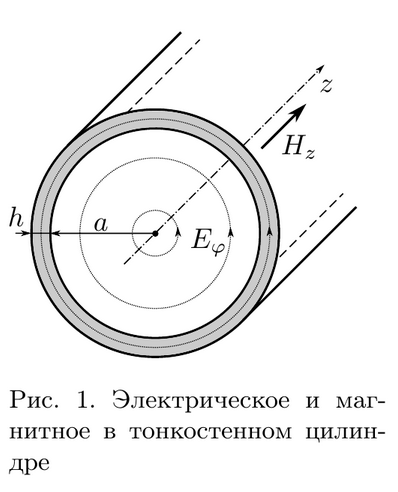
\includegraphics[width=0.8\linewidth]{Screenshot_1}
	\caption{Схема параллельного колебательного контура}
	\label{fig:scheme}
\end{figure}
Зависимость напряжения для конденсатора С $ U(\Omega) $ будет практически такой же, как в последовательном контуре при условии, что импедансы возбуждающей и измеряющей цепей существенно больше, чем импеданс исследуемой цепи. Таким образом,
\begin{equation}
	\frac{1}{\omega C_1}\gg \frac{L}{R C}, \; \; R_O \gg \frac{L}{R C},
\end{equation}
где $ R_O \simeq 1$ \si{\mega \ohm} -- сопротивление на входе осциллографа.

По ширине резонансной кривой определяется добротность контура из формулы:
\begin{equation}
	Q = \frac{\omega_0}{2 \Delta \Omega} = \frac{\nu_0}{\Delta \nu},
	\label{eq:main}
\end{equation}
где $ \omega_0 = 2 \pi \nu_0 $ -- резонансная циклическая частота.

Добротность контура также можно определить по скорости возрастания амплитуды вынужденных колебаний, а также по скорости затухания свободных при резонансном значении частоты (что немаловажно). Обоими этими способами можно воспользоваться, если подавать колебания в контур цугами, то есть отрезками синусоиды в несколько периодов. 

Теоретическое определение резонансной частоты проводится по формуле:
\begin{equation}\label{nu}
	\nu_0 = \frac{1}{2 \pi \sqrt{L C}}
\end{equation}

Для определения добротности применим формулы:
\begin{equation}\label{key}
	\Theta = \frac{1}{n} \ln \frac{U_0 - U_k}{U_0 - U_{k+n}},	
\end{equation}



	\subsection{Эксперементальная установка:}
	
	Схема установки для исследования колебаний приведена на рисунке 2. 
 
 Колебательный контур состоит из постоянной индуктивности {L} с активным сопротивлением $R_{\text{L}}$, переменной емкости {C} и сопротивления {R}. Картина колебаний напряжения на емкости наблюдается на экране осциллографа. Для возбуждения затухающих колебаний используется генератор сигналов специальной формы. Сигнал с генератора поступает через конденсатор $С_{\text{1}}$ на вход колебательного контура. Данная емкость необходима чтобы выходной импеданс генератора был много меньше импеданса колебательного контура и не влиял на процессы, проходящие в контуре. 

 \begin{figure}[h]
	\centering
	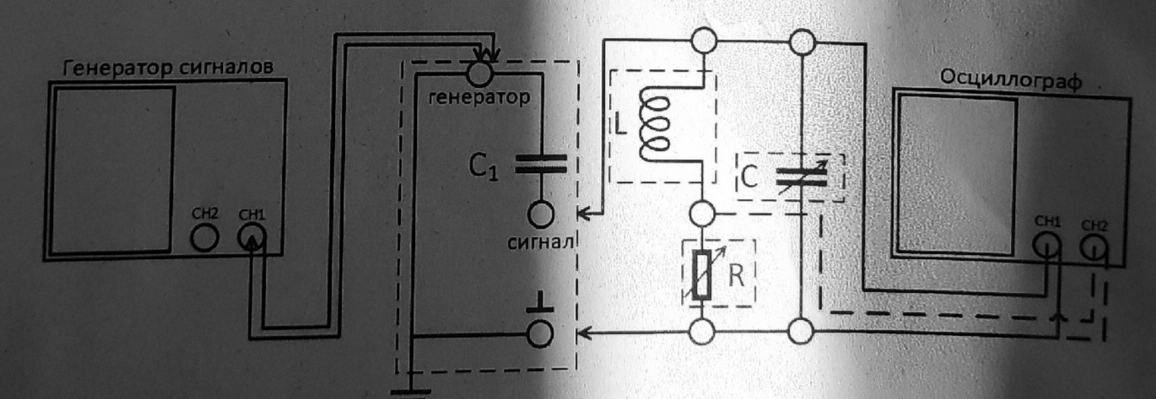
\includegraphics[scale=0.5]{ystanovka.png}
	\caption{Схема установки для исследования свободных колебаний} \label{Device}
\end{figure}


 Установка предназначена для исследования не только возбужденных, но и свободных колебаний в электрической цепи. При изучении свободно затухающий колебаний генератор специальных сигналов на вход колебательного контура подает периодические короткие импульсы, которые заряжают конденсатор $С$. За время между последовательными импульсами происходит разрядка конденсатора через резистор и катушку индуктивности. Напряжение на конденсаторе $U_{\text{C}}$ поступает на вход канала 1($X$) электронного осцилографа. Для наблюдения фазовой картины затухающих колебаний на канал 2($Y$) подается напряжение с резистора $R$ (пунктирная линия на схеме установки), которое пропорционально току $I$ ($I\propto\frac{\text{d}U_C}{\text{d}t}$).

 При изучении возбужденных колебаний на вход колебательного контура подается синусоидальный сигнал. С помощью осциллогрофа возможно измерить зависимость амплитуды возбужденных в зависимости от частоты внешнего сигнала, из которого возможно определить добротность колебательного контура. Альтернативным способом расчёта добротности контура является определение декремента затухания по картине установления возбужденных колебаний. В этом случае генератор сигналов используется для подачи цугов синусоидальной формы. 
  
	\section{Ход работы}
 \subsection{Подготовка приборов к работе:}
 Подключив генератор специальных сигналов ко входу 1($X$) осциллогрофа и установив на нём последовательность импульсов, мы убедились, что на осцилографе отображаются периодические импульсы, добившись статичной картины сигнала мы собрали схему согласно рисунку 2. 

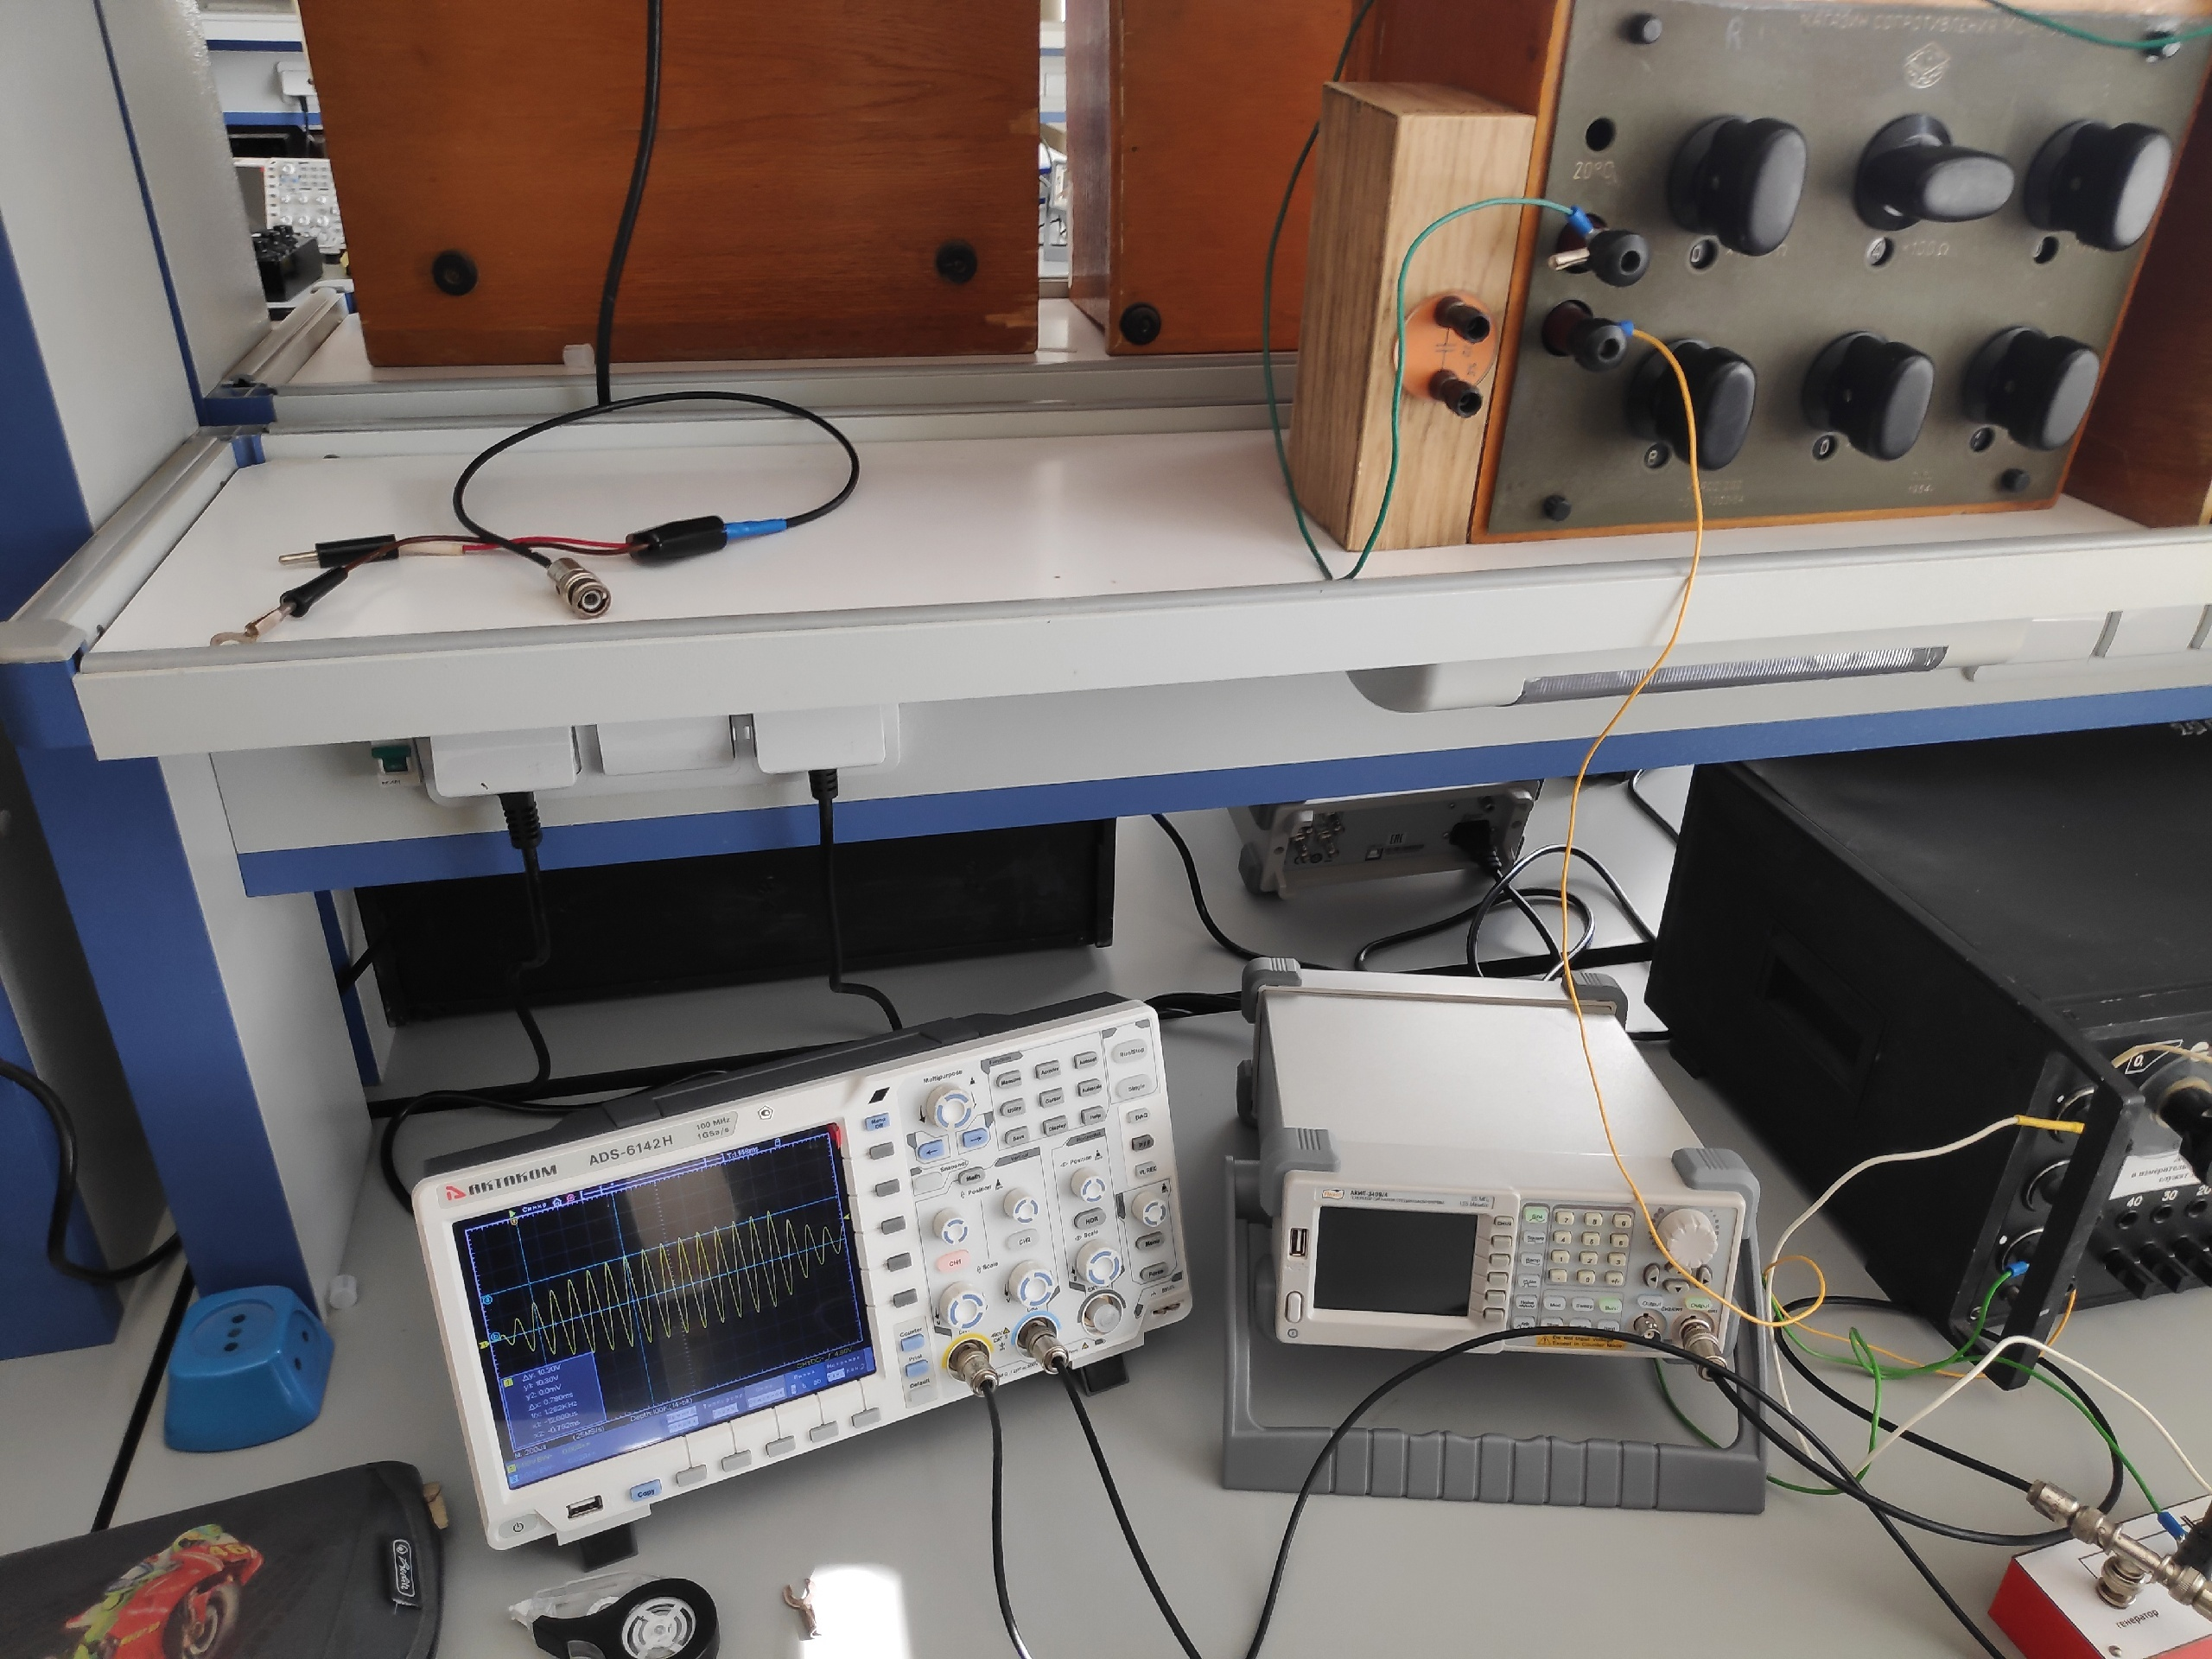
\includegraphics[width=0.48\linewidth]{Photo1.jpg}
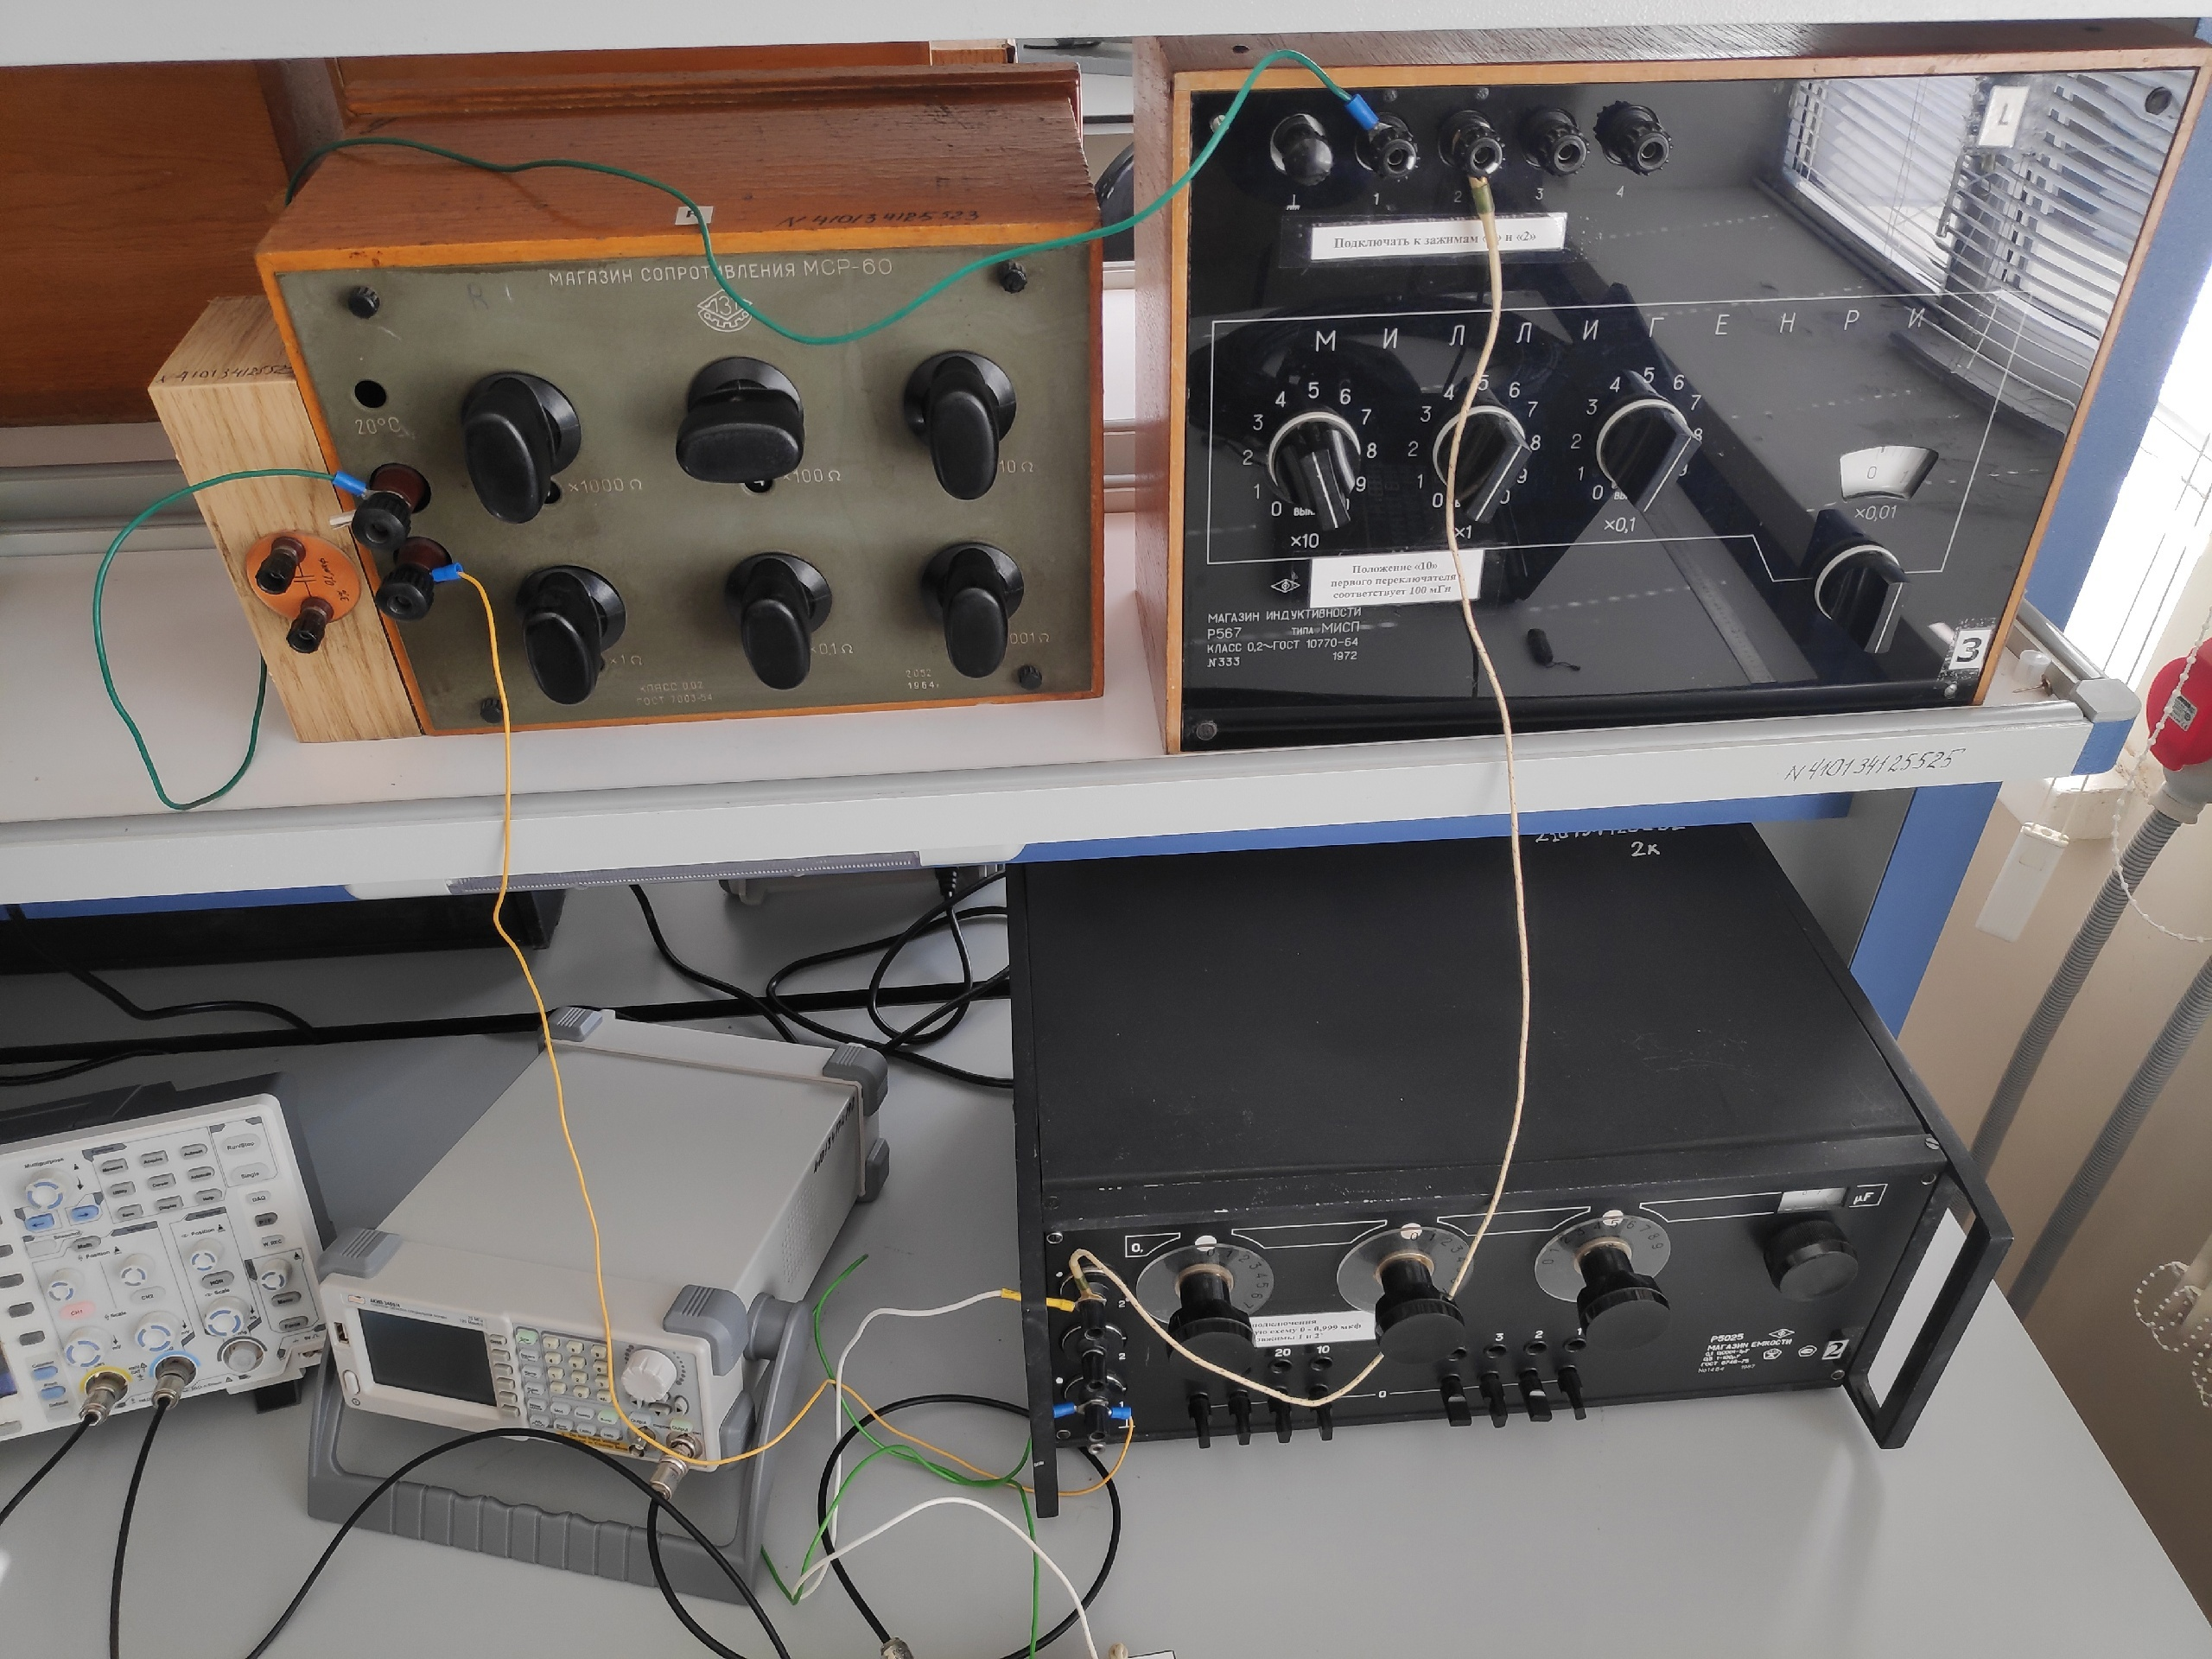
\includegraphics[width=0.48\linewidth]{Photo 2.jpg}

\newpage
 \subsection{Измерение периодов свободных колебаний:}
 \begin{enumerate}

\item Установив все необходимые значения велечин на установке: $R = 0\;{Ом}$, $L = 100\;{мГн}$ и $C = 0\;{мкФ}$, мы получили картину свободно затузающих колебаний. 
 
 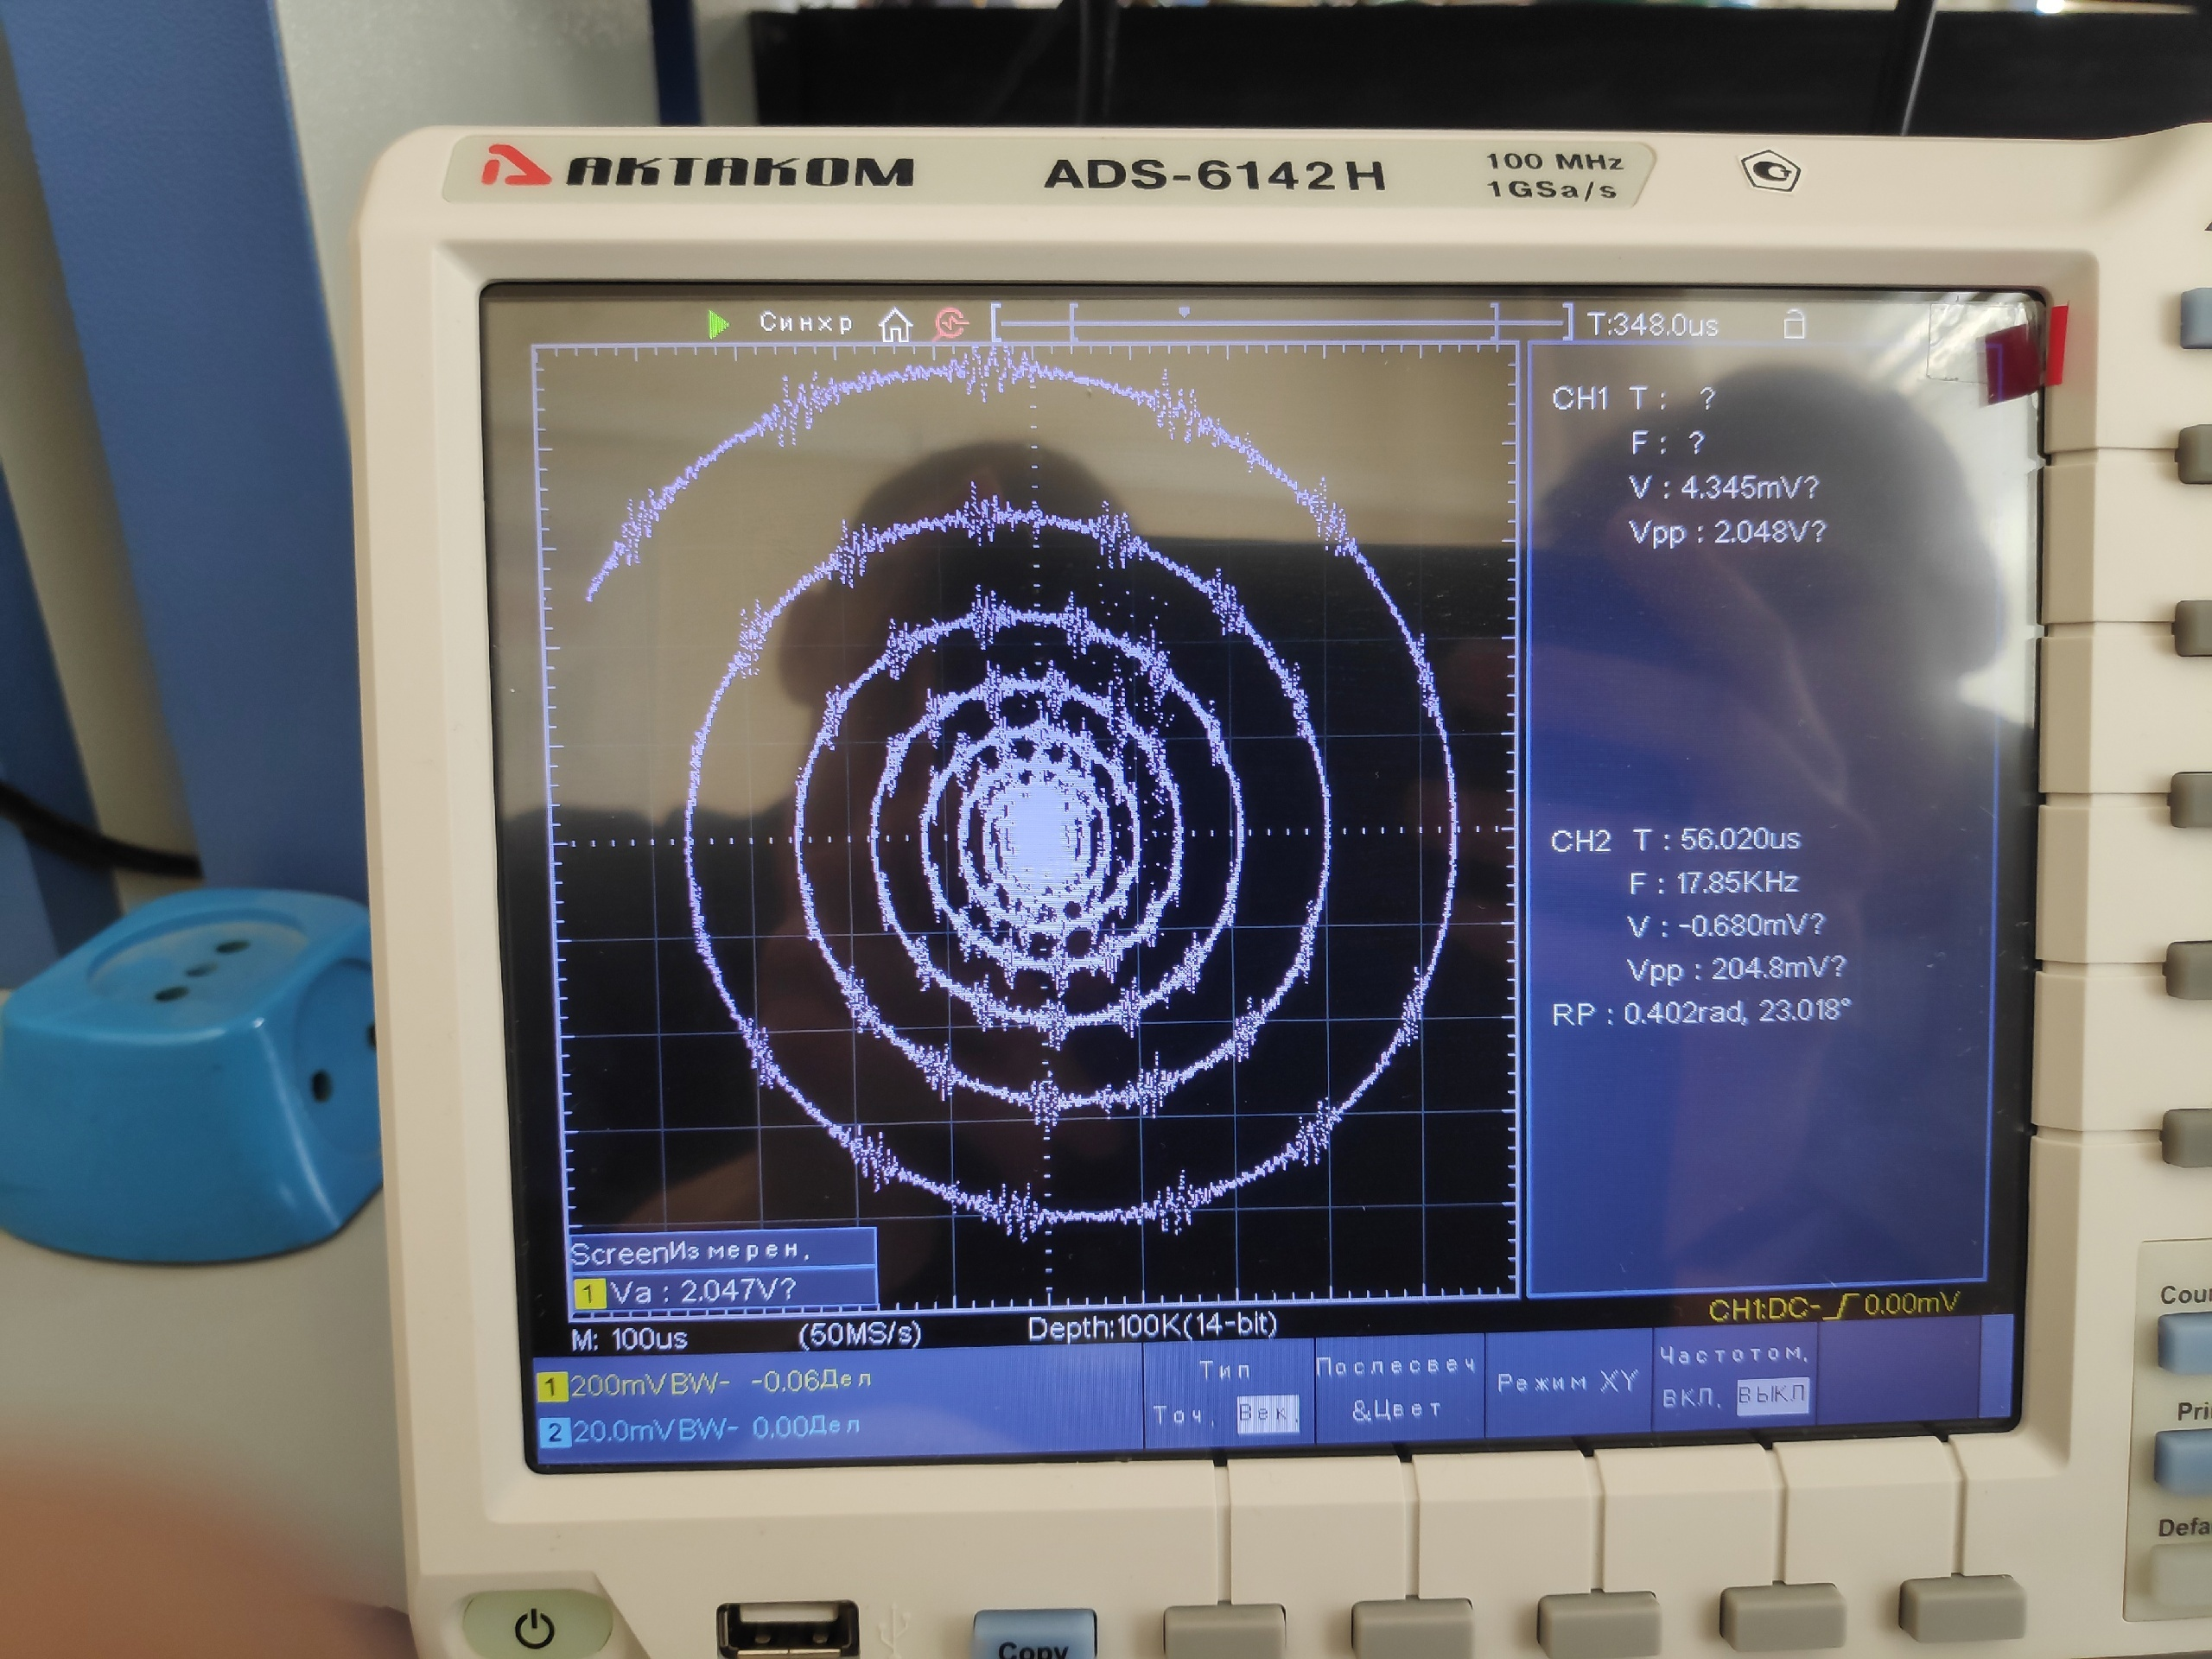
\includegraphics[width=0.6\linewidth]{Spiral.jpg}

 \item По периоду колебаний для $C = 0\;мкФ$ мы определили нулевую ёмксоть используя формулы: &{T_1=\frac{2\pi}{\omega_1}}& $ и $  $\omega_1=\sqrt{\frac{1}{LC_o}-\frac{R^2}{4L^4}}$, где получили $C_o = 0.001 \; мкФ$

 \item Изменяя емкость по курбелям с учётом нулевой емкости получаем таблицу значений и занесём в таблицу также значения периода, рассчитанные по теоретической формуле $T=2\pi\sqrt{LC}$: 
 \begin{table}[h]
	\centering
	\begin{tabular}{|c|c|c|c|c|c|c|c|c|c|c|}
		\hline
		$C$,мкФ&0,001&0,003&0,005&0,007&0,010\\ \hline
		$n$&6&12&9&8&12\\ \hline
		$t$,мс&0,41&1,344&1,292&1,348&2,208\\ \hline
		$T$,мс&0,068&0,112&0,144&0,169&0,200\\ \hline
            ${T_{th}}$,мс&0,063&0,109&0,140&0,166&0,199\\ \hline
	\end{tabular}
 \caption{Зависимость периода $T$ затухающих колебаний от ёмкости $C$} \label{per}
\end{table}

Видим, что значения $T$ и $T_{th}$ очень точно совпадают в пределах погрешностей, что говорит о точности исходных измерений.

\item Построим График зависимости $ T(T_{th})$.
	\begin{center}
			\begin{tikzpicture}[scale = 0.8]
			\begin{axis}[
			axis lines = left,
			legend style={at={(1,0.3)}},
			xlabel = {$T$, {мc * 10^{-3}}},
			ylabel = {$T_{th}$, {мc * 10^{-3}}},
			xmin=0, xmax=200,
			ymin=0, ymax=200,
			ymajorgrids = true,
			xmajorgrids = true,
			minor tick num = 4
			]
			\addplot+[only marks ] plot[error bars/.cd, y dir=both, y explicit]
			coordinates {
				(68,63)
				(112, 109) 
				(144, 140)
				(169, 166)
				(200 , 199)
			};
			\addplot[red, domain=0:200]{-5+1.01*x};
			\legend{
				$С помощью \; МНК$, $k = 1.008 \pm 0.001 $
			};
 			\end{axis}
			\end{tikzpicture}
		\end{center}
 
\end{enumerate}

\newpage

 \subsection{Критическое сопротивление и декремент затухания:}

 
	\begin{enumerate}
		\item Приняв $L=100~\text{мГн}$, рассчитаем ёмкость $C*$, при которой собственная частота колебаний контура $\nu_0=\frac{1}{2\pi\sqrt{LC}}$ составит 6.5 кГц. Получим значение $C* =\frac{1}{4\pi^2\nu_0^2L}=0,00599~\text{мкФ}$. Учитывая расчитанную ранее нулевую емкость получаем, что выставленное значение на магазине будет равно 5 мкФ. Рассчитаем также критическое сопротивление контура с такими параметрами, оно равно $R_{\text{кр}}=4\pi\nu_0L=8168~\Omega$.
  
  \item Установим на магазине ёмкость $C=0,005~\text{мкФ}$. Будем увеличивать сопротивление $R$ от нуля до $R_{\text{кр}}$, наблюдая картину затухающих колебаний на экране ЭО. Колебательный режим переходит в апериодический примерно при $R_{\text{кр}}=8168~\Omega$, будем в дальнейшем использовать его.

  \item Приступим к измерению логарифмического декремента затухания. Установим сопротивление $R=0,05R_{\text{кр}}=408~\Omega$. Получим на экране ЭО картину колебаний. Проведём измерения для 5 различных значений $R$ в диапазоне от $0,05R_{\text{кр}}$ до $0,25R_{\text{кр}}=2042~\Omega$. Логарифмический декремент затухания находится по формуле\[\Theta=\frac{1}{n}\ln{\frac{U_m}{U_{m+n}}}.\] Занесём все результаты в таблицу 2.

  \begin{table}[h]
	\centering
	\begin{tabular}{|c|c|c|c|c|c|c|c|c|}
		\hline
		$\frac{R}{R_{\text{кр}}}$ & 0,05 & 0,09 & 0,13 & 0,17 & 0,21\\ \hline
		$R,\ \Omega$ & 408 & 735 & 1062 & 1388 & 1715 \\ \hline
		$U_m$, мВ & 784 & 652 & 544 & 456 & 760 \\ \hline
		$U_{m+n}$, мВ & 76 & 56 & 40 & 44 & 48 \\ \hline
		$n$ & 7 & 4 & 3 & 2 & 2  \\ \hline
		$\Theta$ & 0,33 & 0,61 & 0,87 & 1.17 & 1.38 \\ \hline
  $X,\ 10^{-7}\Omega^{-2}$ & 54.6 & 17.5 & 8.54 & 5.05 & 3.32\\ \hline
  $Y$ & 9.18 & 2.69 & 1.32 & 0,73 & 0,53 \\ \hline
	\end{tabular}
 \caption{Зависимость логарифмического декремента затухания $\Theta$ от сопротивления контура $R$} \label{decr}
\end{table}

\item В дальнейшем нам подсказал лаборант, что в работе активное омическое сопротивление витков катушки при 5 кГц, равно около $R_L= \; 20\Omega$. Видим, что тогда при вычислении $R_{\Sigma}=R+R_L$.

Приняв обозначения $X=\frac{1}{R_{\Sigma}^2}$ и $Y=\frac{1}{\Theta^2}$, можно показать, что $R_{\text{кр}}=2\pi\sqrt{\frac{\Delta Y}{\Delta X}}$. Вычислим величины $X$ и $Y$ тоже занесём в таблицу.

Построим график $Y(X)$: 

 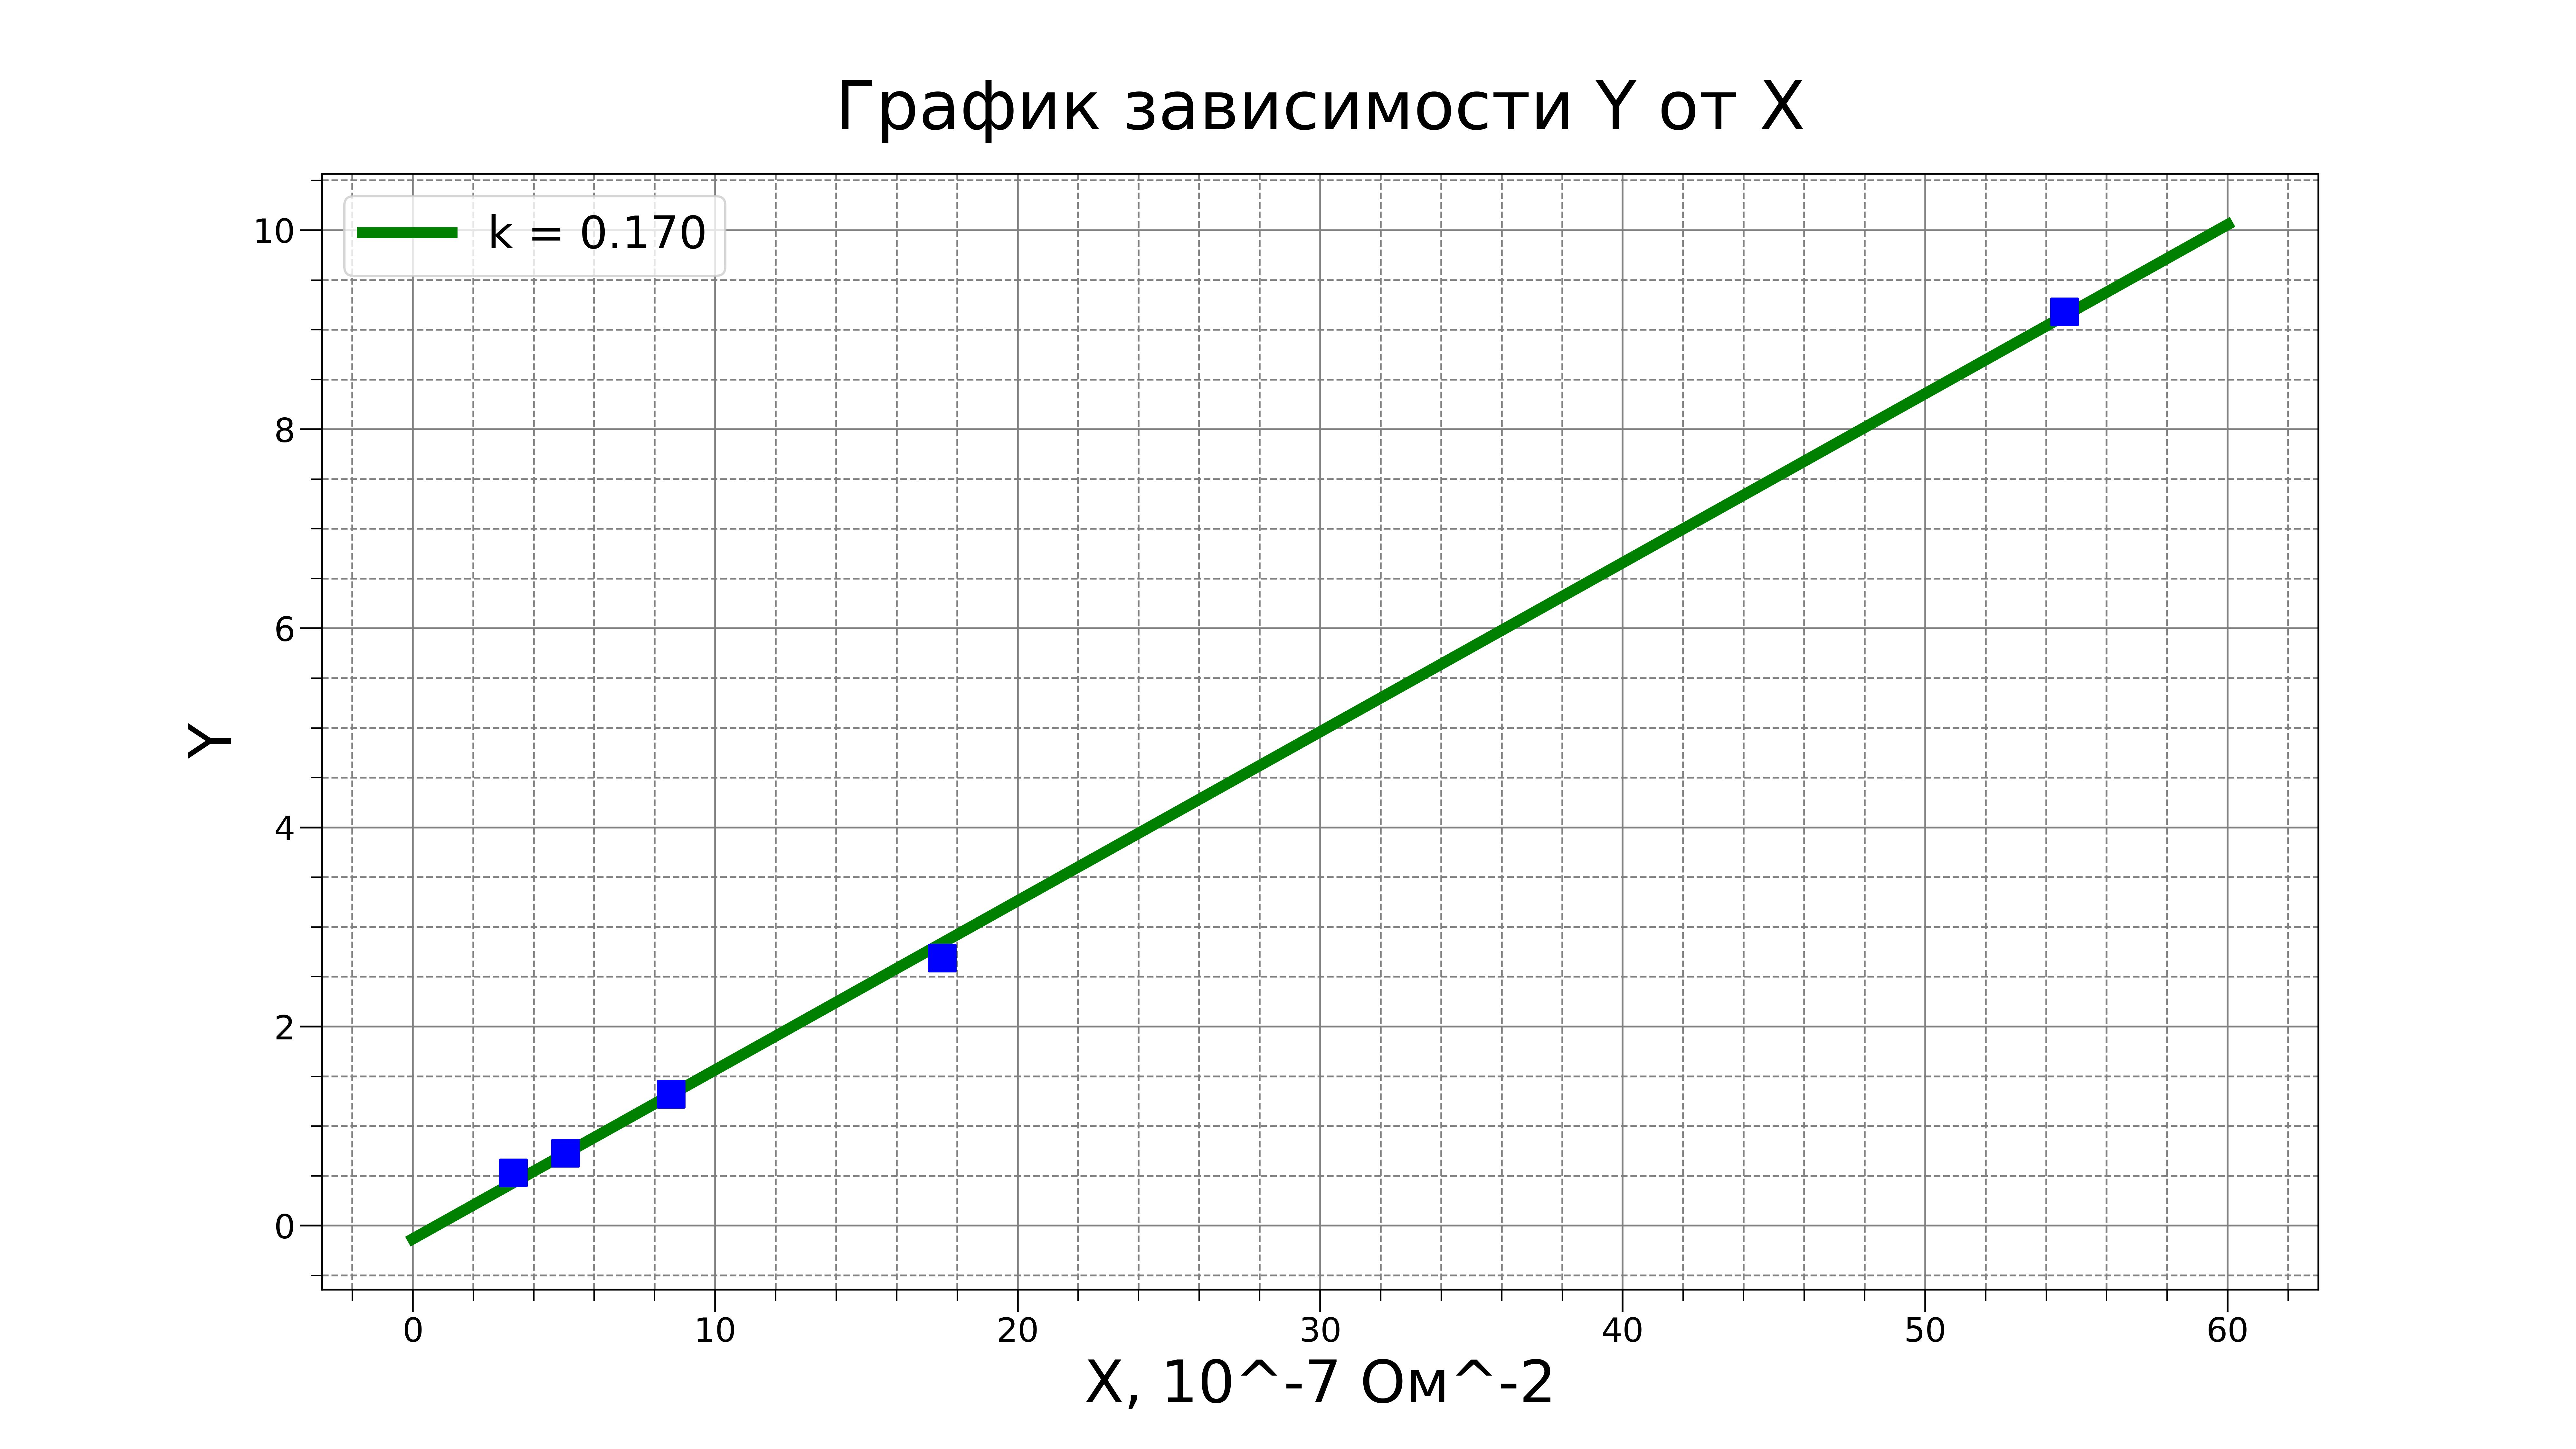
\includegraphics[width=0.6\linewidth]{Graph.jpg}
 
 Непосредственно из графика находим $\frac{\Delta Y}{\Delta X}=\left(1,70\pm0,002\right)\cdot10^6~\Omega^2$, откуда находим $R_{\text{кр}}=\left(8192\pm48\right)~\Omega$. Видим, что при этом определить критическое сопротивление по точке пересечения графика с осью абсцисс в какой бы то ни было вменяемой точностью практически невозможно.

Теоретическое значение критического сопротивления $R_{\text{кр}}=2\sqrt{\frac{L}{C}}=\left(8168\right)~\Omega$, т.е. в пределах погрешности оно совпадает с полученным в эксперименте.

\item Мы зафиксировали два значения сопротивления: $R_1=0,05R_{\text{кр}}=408~\Omega \; и \; R_2=0,09R_{\text{кр}}=735~\Omega.$ Однако 2-ое значение сопротивления мы взяли слишком маленькое по невнимательности. 
\end{enumerate}
\subsection{Свободные колебания на фазовой плоскости:}
\begin{enumerate}
\itemПереключим ЭО на двухканальный режим для одновременного наблюдения осциллограмм тока и напряжения. Подберём масштабы и частоту развёртки так, чтобы оба сигнала были представлены на временном интервале, слегка превышающем период повторения импульсов с генератора. Полученная картина будет качественно совпадать с показанной на рисунке.

\itemДля наблюдения затухающих колебаний на фазовой плоскости переключим развёртку ЭО в положение $X-Y$. На магазине сопротивлений выберем значение $R=0,5R_{\text{кр}}$. Подберём масштаб спирали и частоту импульсов генератора(400Гц), удобный для измерений. Спираль качественно совпадает с теоретической.

\itemПри том же значении $C$, что и в части II Хода работы, пронаблюдаем за изменением спирали при увеличении сопротивления от 0,05 до 0,25$R_{\text{кр}}$. Видим, что спираль закручивается слабее и становится менее плотной с ростом $R$.

Для определения $\Theta$ измерить координаты пересечения витков спирали с осью координат не удалось, в следствии низкой точности измерения координат по шкале осциллографа. Поэтому мы внесём в таблицу значения добротности контура, рассчитанное теретически из величин его параметров по формуле приблежения: \[Q={\frac{1}{R}}\cdot\sqrt{\frac{L}{C}},\] а также значения минимальной и максимальной добротности, вычисленные по формуле\[Q=\frac{\pi}{\Theta},\].

\begin{table}[h]
	\centering
	\begin{tabular}{|c|c|c|c|c|c|c|c|}
		\hline
		$\frac{R}{R_{\text{кр}}}$ & $\Theta$ & $Q_{th}$ & $Q$ \\ \hline
		 0.05  & 0.33 & 10 & 9.51\\ \hline
		 0.09  & 0.61 & 5.55 & 5.15\\ \hline
          0.13  & 0.87 & 3.84 & 3.61\\ \hline
          0.17  &  1.17& 2.94 &2.69\\ \hline
          0.21  &  1.38& 2.38 & 2.28\\ \hline
	\end{tabular}
 \caption{Зависимость добротности контура $Q$ от сопротивления $R$} \label{lst}
\end{table}

\newpage

 \subsection{Исследование резонансных кривых:}
Теоретическое определение резонансной частоты проводится по формуле:
	$\nu_0 = \frac{1}{2 \pi \sqrt{L C}} = 6.5 \; кГЦ $
 а экспериментально $\nu_0* = 6.41 \; кГЦ $ и ${U_c}=11.5\; В$

Результаты исследования резонансных кривых отображены в таблице \ref{tabb}, по которым был построен график на рис. \ref{fig:graph} в безразмерных координатах:



\begin{table}[h]
	\centering
	\begin{tabular}{|l|l|l|l||l||l|}
		\hline
		\multicolumn{3}{|l|}{\textbf{R=408 Ом}}         & \multicolumn{3}{l|}{\textbf{R=735 Ом}}        \\ \hline
		\textbf{Частота, Гц} & \textbf{Напряжение, В} & \textbf{Сдвиг, мкс} & \textbf{Частота, Гц} & \textbf{Напряжение, В} & \textbf{Сдвиг, мс}\\ \hline
		5700                 & 4.6                           &  72       & 5870                 & 4.76                      &    57.2      \\ \hline
		5870                 & 5.8                         &      68     & 6040                 & 5.64                       &    50.4      \\ \hline
		6040                 & 7.6                         &      60     & 6210                 & 6.36                       &     43.2   \\ \hline
		6210                 & 9.7                         &     50      & 6380                 & 6.84                       &     35.6     \\ \hline
		6380                 & 11.2                         &     37.2   & 6550                 & 6.88                       &     29.2     \\ \hline
		6550                 & 10.8                        &      26.8   & 6720                 &   6.44                     &    22.4      \\ \hline
		6720                 & 9.2                        &      18.8    &                  &                   &          \\ \hline
		6890                 & 7.6                         &     13.6    &                 &                     &          \\ \hline
		7060                 & 6.4                        &      10      &                  &                          &          \\ \hline
		7230                 & 5.6                         &      8      &                    &                       &          \\ \hline
	\end{tabular}
	\caption{Исходные данные для резонансных кривых}
	\label{tabb}
\end{table}

 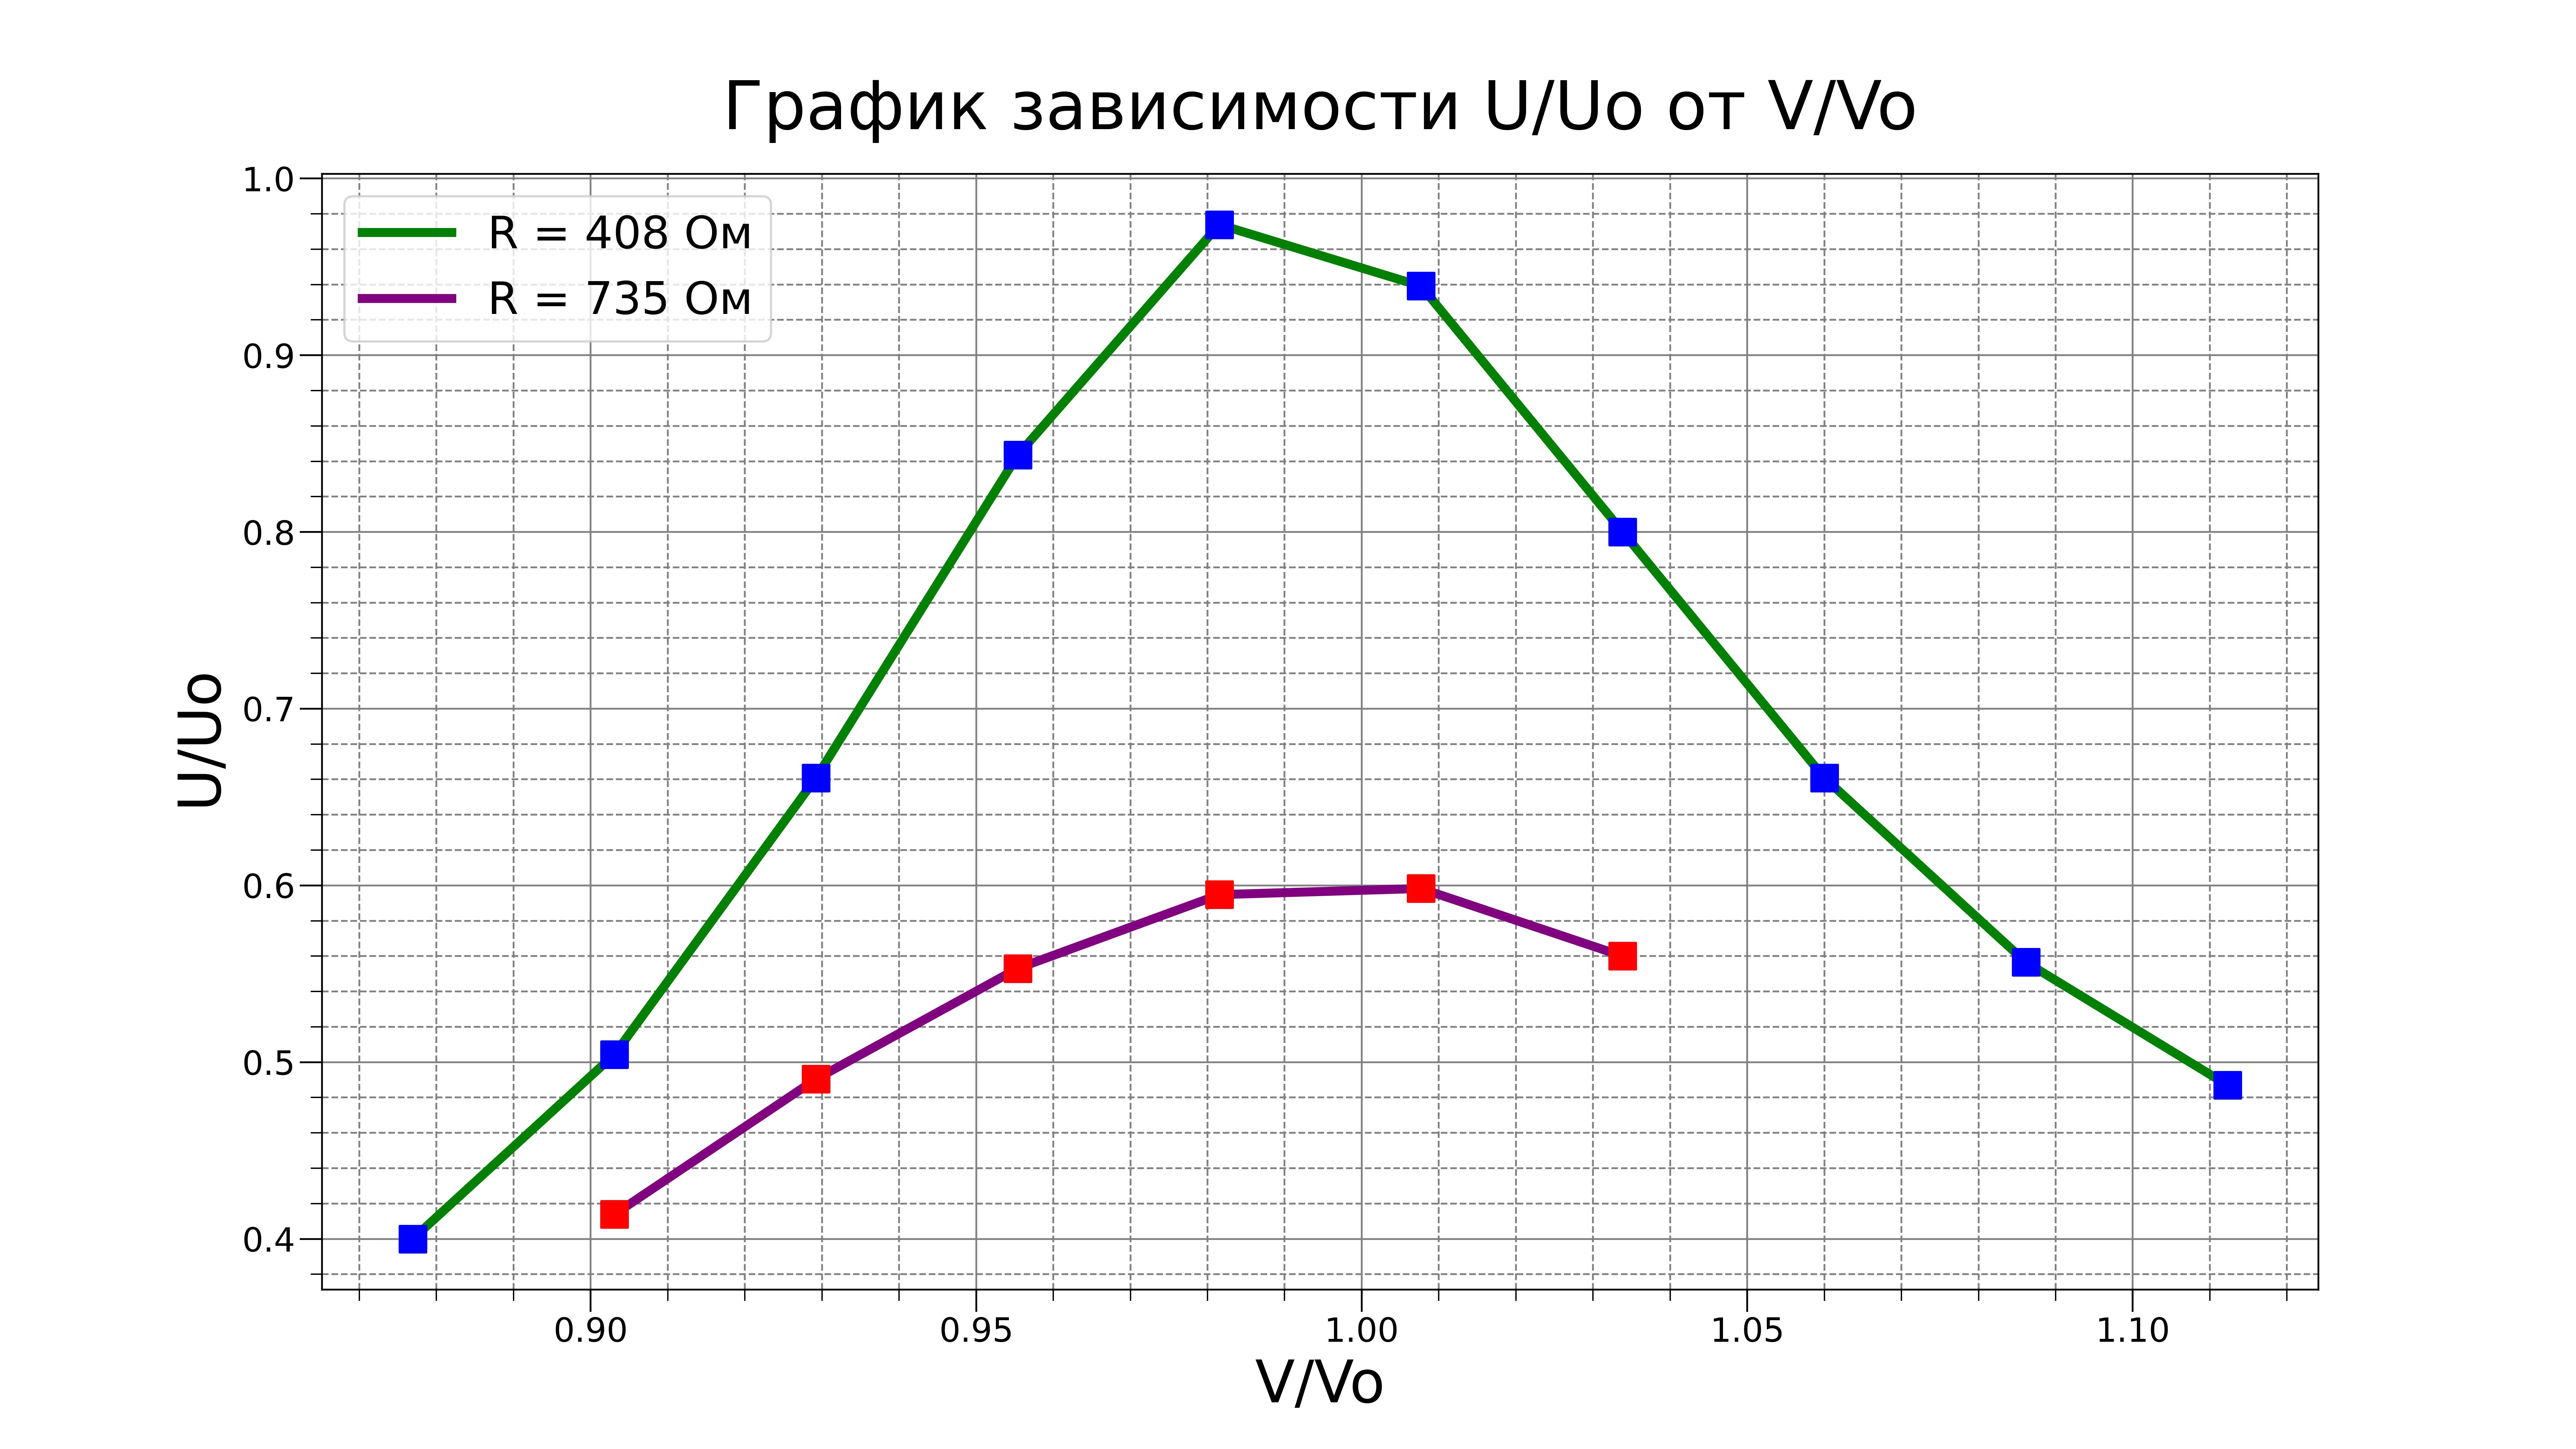
\includegraphics[width=1\linewidth]{graphikmoy.jpg}


Из графика мы находим ширину резонансной кривой равную: $2{\Delta\Omega } =\;0.115 $ Для R = 408 Ом, и ${\Delta\Omega } =\;0.1 $ Для R = 735 Ом.
Добротности в таком случае равны:

$ Q_{R=408} = 55,$
$ Q_{R=735} = 63 $
\newpage
\subsection{Процессы установления и затухания:}
Выставляем на генераторе цугов
эту частоту, и подбираем длительность и период цегов так, чтобы колебания успели
установится и затухнуть соответственно.
Мы успели снять только одно значение: 
$ {\Theta = \frac{1}{n} \ln \frac{U_0 - U_k}{U_0 - U_{k+n}} = \frac{1}{5} \ln \frac{11 - 5.8}{11 - 10.3}} = 0.4	$

 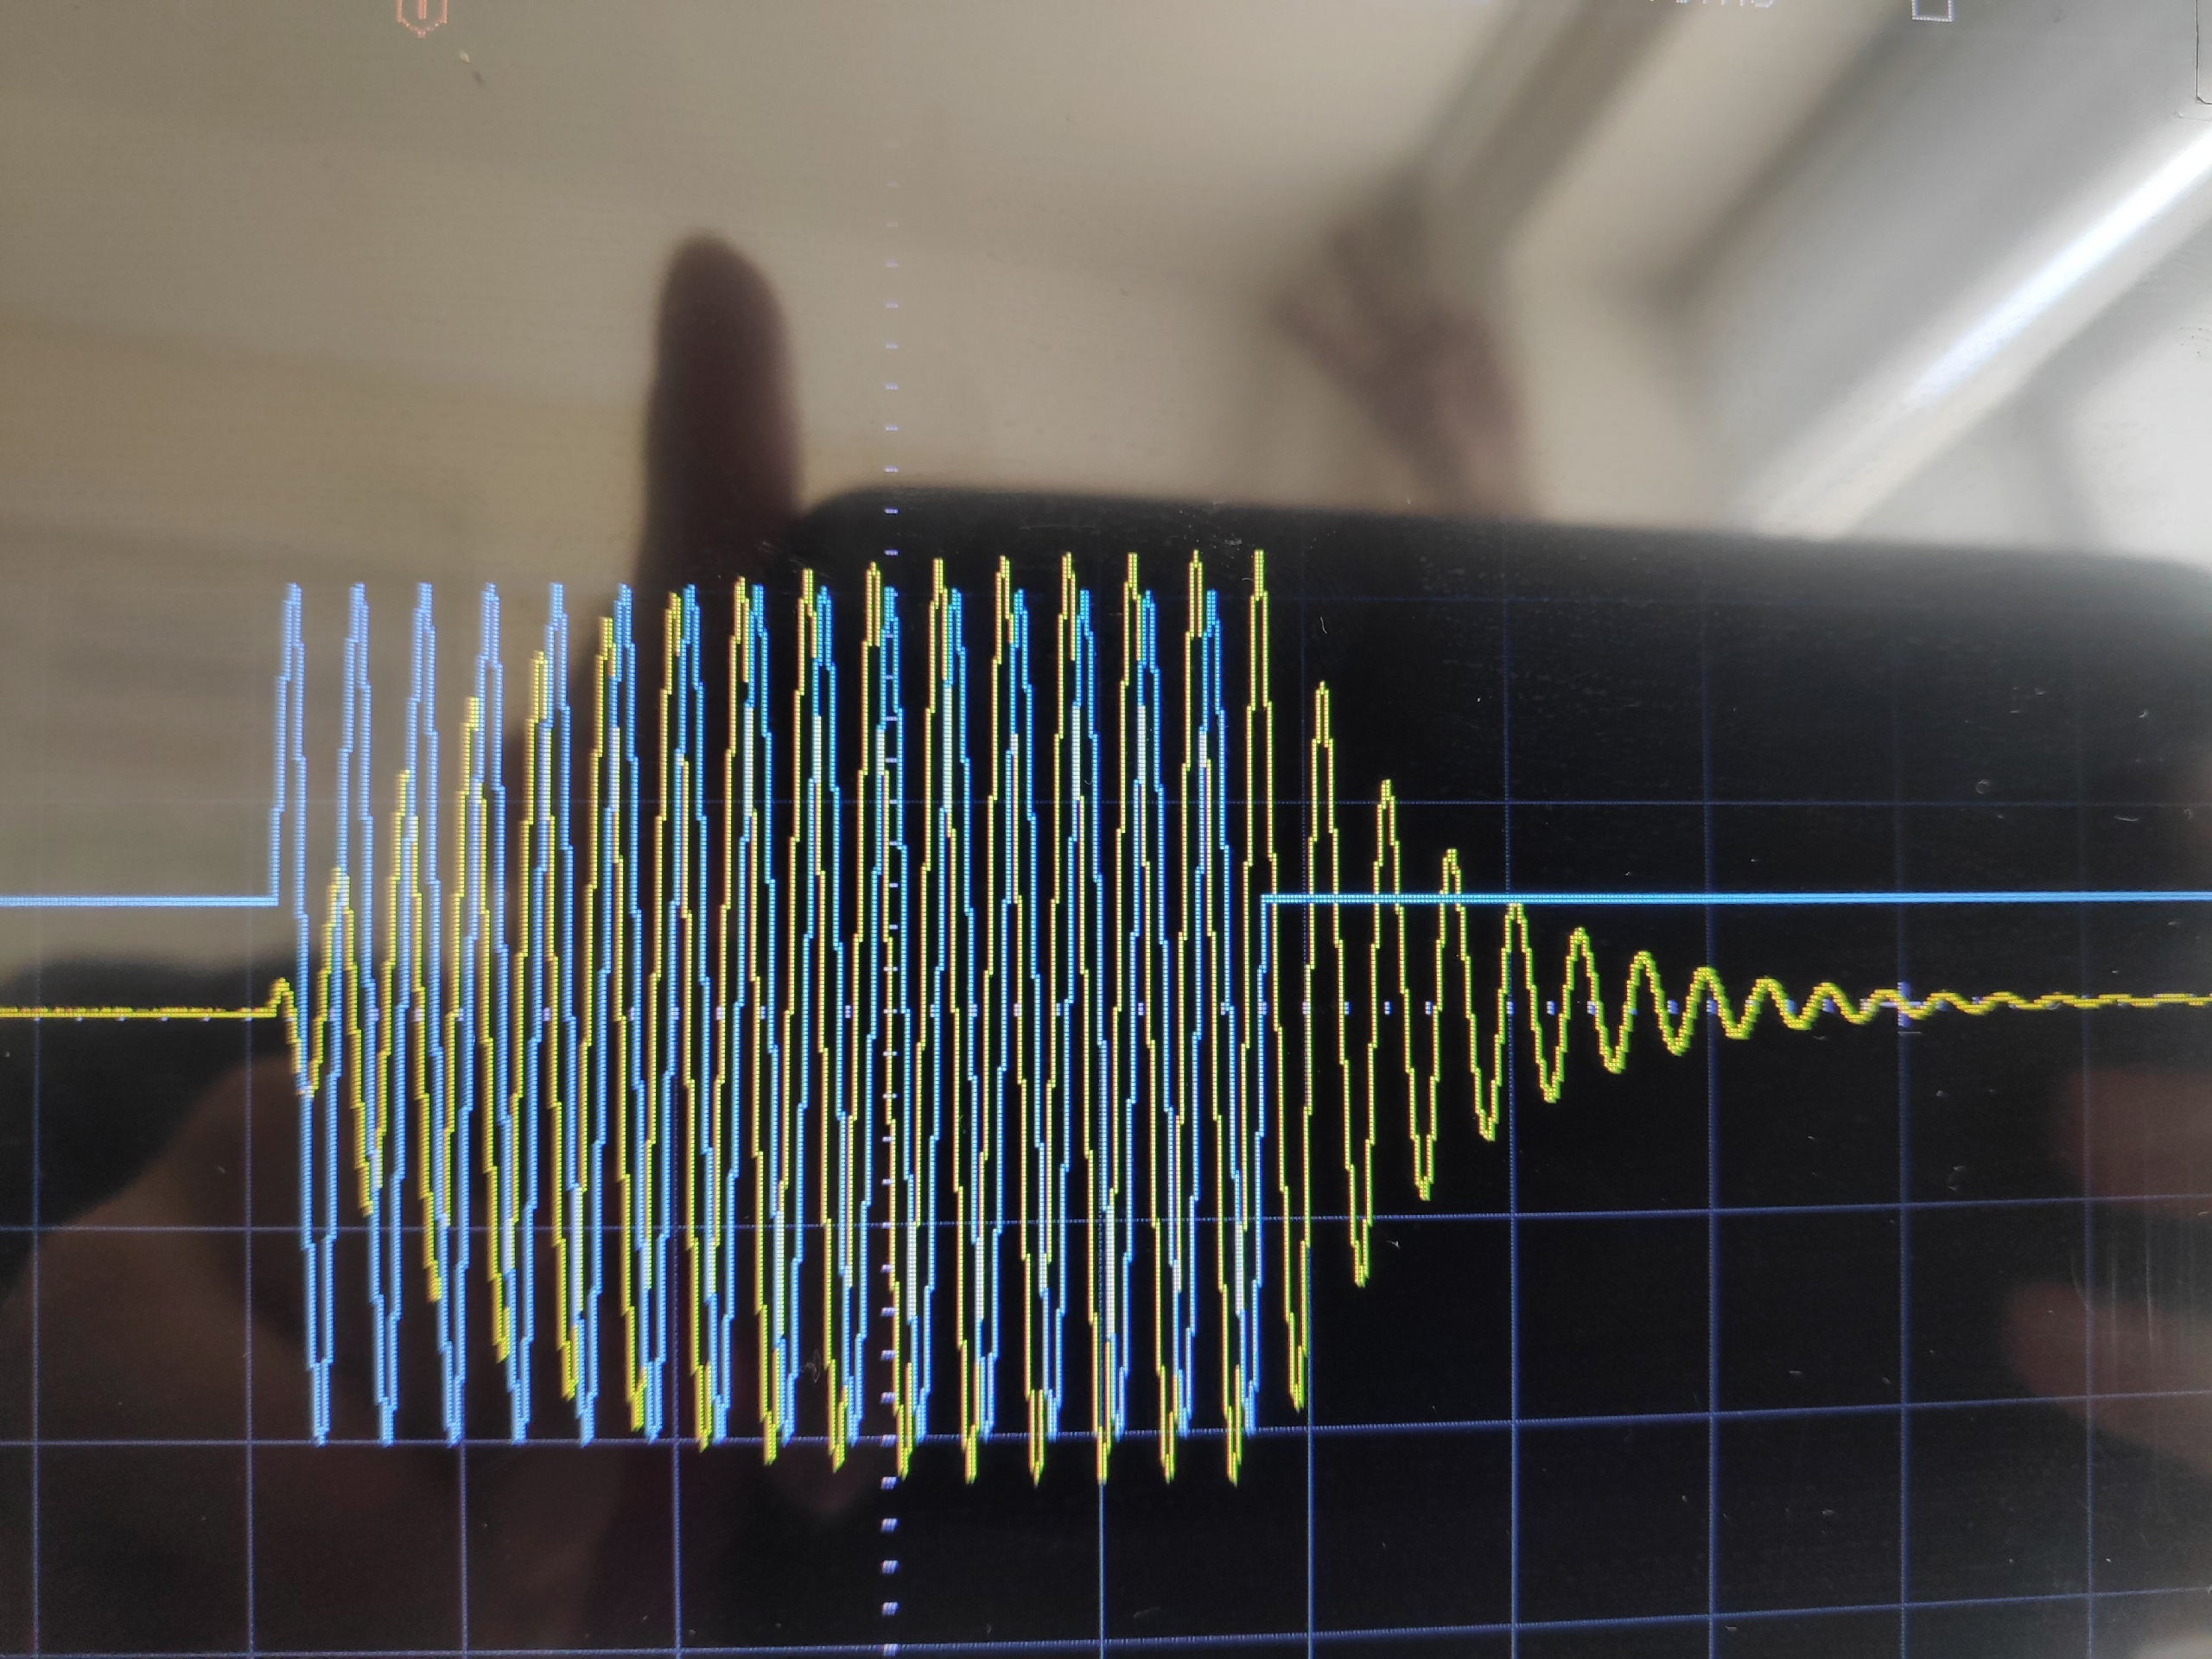
\includegraphics[width=0.7\linewidth]{Abama.jpg}

\section{Вывод:}

\begin{table}[h!]
	\centering
	\begin{tabular}{|l|l|l|l|l|}
		\hline
		R      &$f(LRC)$ & $f(\Theta)$         & АЧХ      & Нарастание      \\ \hline
		408 ОМ & 10      & 9.51                & 55      & 0.4   \\ \hline
		735 Ом & 5.55    & 5.15                & 63      & -   \\ \hline
	\end{tabular}
	\caption{Результаты измерения добротности}
	\label{1}
\end{table}

В данной работе были исследованы свободные и вынужденные колебания в электрическом колебательном контуре.

В первой части работы был измерен период свободных затухающих колебаний, и экспериментально с высокой точностью была подтверждена соответствующая теоретическая зависимость.

Также был измерен декремент затухания контура. С его помощью было найдено критическое сопротивление контура $R_{\text{кр}}=\left(8192\pm48\right)~\Omega$, в пределах погрешности совпадающее с теоретически предсказанным $R_{\text{кр}}=\left(8168\right)~\Omega$, что говорит о точности используемого метода.

Однако не все методы оказались споставимы по точности, большое разхождение в значениях произошло в АЧХ методе из-за малого кол-ва точек собраных нами при эксперементе. Ещё одна из ключевых ошибках, взятие небольшого диапозона частот в методах с вынужденными колебаниями, мы взяли {R_2} = 735 Ома, а не 2000 Ом.

В данной работе хотелось бы улучшить точность измерения добротности с помощью метода измерения координат на фазовой плоскости, чтобы пересечение спирали с осями можно было фиксировать теми же курсорами в осциллографе. 
\end{enumerate}
\end{document}